\documentclass{article}
\usepackage{graphicx}
\usepackage{listings}

\lstset{
	basicstyle=\ttfamily,
	inputpath=../src
}

\begin{document}

\title{Problem 1: System calls, error checking, and reporting}
\author{Caleb Zulawski}

\maketitle

\section{Implementation}

\begin{lstlisting}
$ ./copycat -h
Usage: copycat [OPTION]... [FILE]...
Concatenate FILE(s), or standard input, to standard output.
Similar to GNU cat.

  -v           print diagnostic messages to standard error
  -b SIZE      size of internal copy buffer, in bytes
  -m MODE      file mode, in octal
  -o FILE      output to FILE instead of standard output
  -h           display this help and exit
\end{lstlisting}

This software was developed and tested on Linux 3.10.18 on an x86-64 netbook.
The buffer size dependent performance is shown in Figure \ref{performancefig}.
The higher performance for larger buffers indicates that reading into and writing from the buffer is very fast compared to the process of setting up the read() or write().
The larger buffers seem to have similar performance because there is virtually no overhead compared to the amount being written.

\section{Examples}

\subsection{Basic use}

\begin{lstlisting}
$ ./copycat 
Hello World
Hello World
EOF
$
\end{lstlisting}

\subsection{Concatenating from standard input and a file}

\begin{lstlisting}
$ echo And again... | ./copycat - copycat.c
And again...
/* copycat.c
 * Caleb Zulawski
 * 
 * Entrance point of the program.
 */

#include "copycat.h"

int main(int argc, char* argv[]) {
    Options options;
    
    cc_parse_args(argc, argv, &options);
    cc_log(&options);
    cc_copy(&options);

    return 0;
}
$
\end{lstlisting}

\subsection{Writing to a file, with error handling}

\begin{lstlisting}
$ touch outfile
$ chmod 000 outfile
$ echo nope | ./copycat -o outfile -
Error opening file outfile: Permission denied
$ sudo chmod 644 outfile
$ echo yup | ./copycat -o outfile -
$ cat outfile
yup
$
\end{lstlisting}

\subsection{Bad input file behavior}
\begin{lstlisting}
$ echo Uh oh | ./copycat - nofile
Uh oh
Error opening file nofile: No such file or directory
$ echo Uh oh | ./copycat nofile -
Error opening file nofile: No such file or directory
$ 
\end{lstlisting}

\begin{figure}
    \centering
    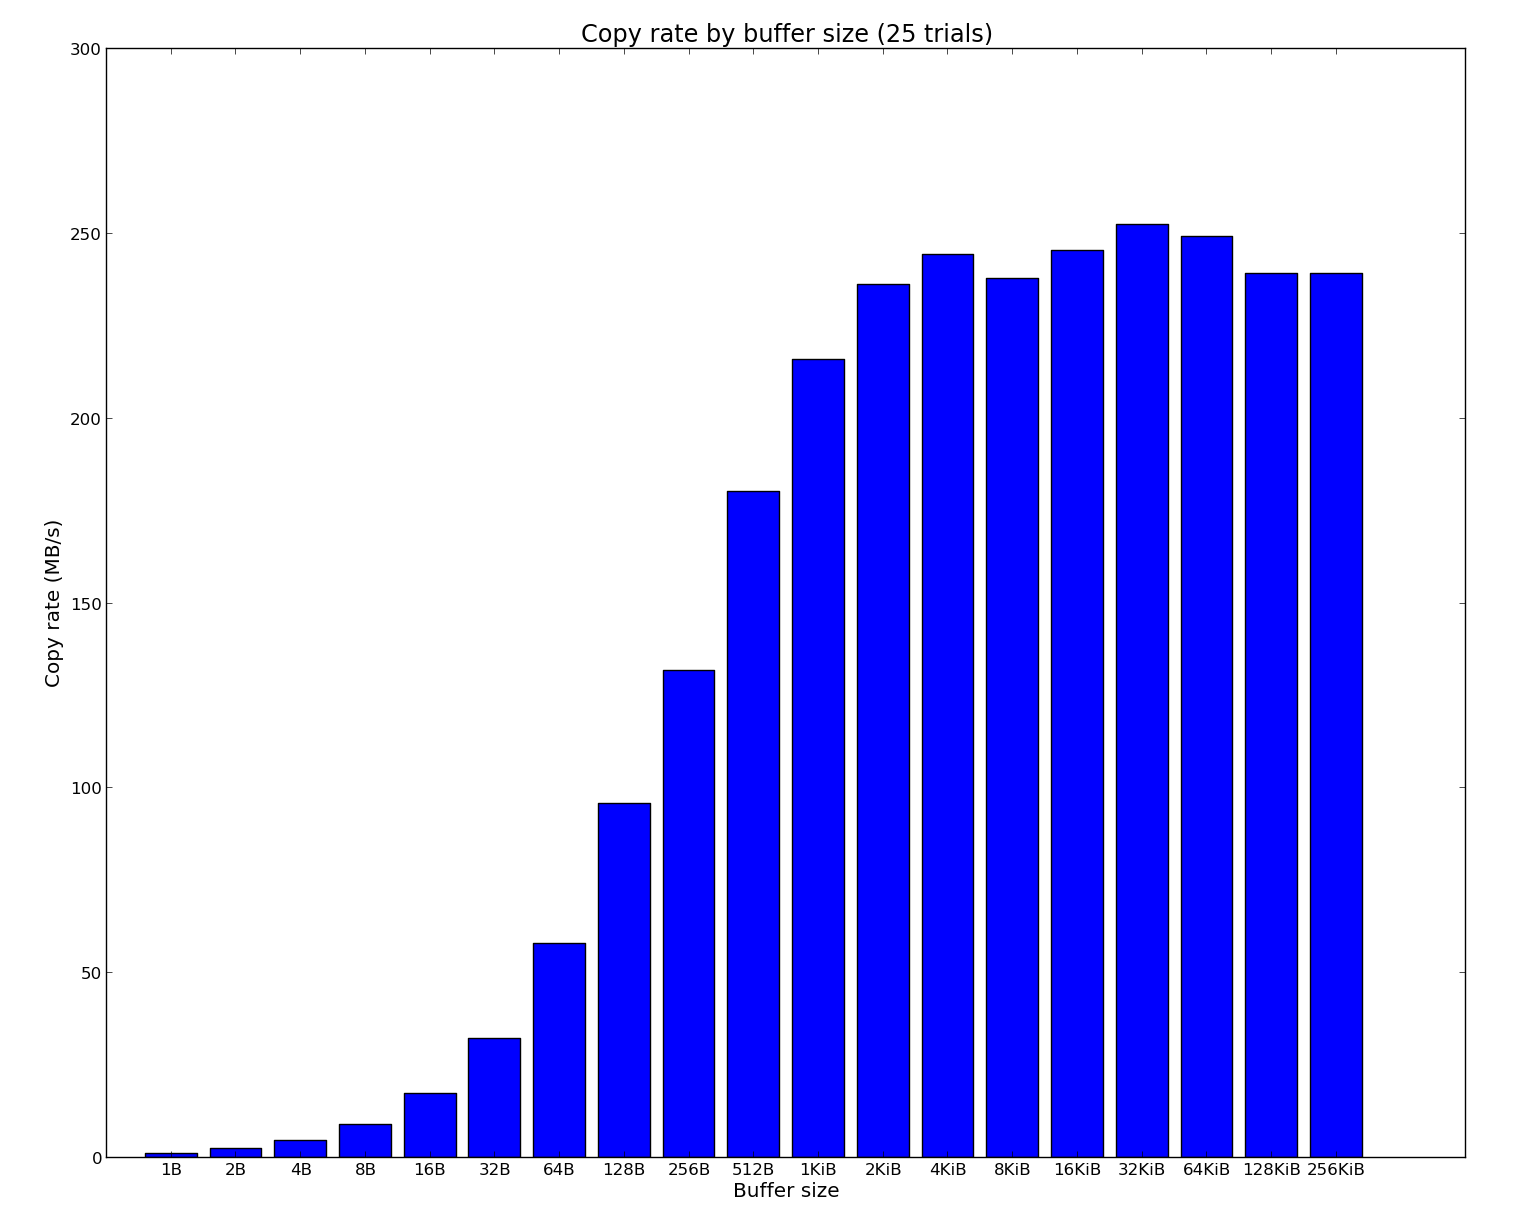
\includegraphics[width=\linewidth]{../test/results}
    \caption{Performance}
    \label{performancefig}
\end{figure}


\end{document}